\chapter{Конструкторский часть}

В данном разделе будут представлены требования к разрабатываемому программному обеспечению, описание используемых типов данных, а также схемы алгоритма полного перебора и муравьиного алгоритма.

\section{Описание используемых типов данных}
При реализации алгоритмов будут использованы следующие типы дан-
ных:
\begin{itemize}[label=---]
	\item размер матрицы смежности --- целое число;
	\item имя файла --- строка;
	\item коэффициенты $\alpha, \beta$, \textit{k\_evaporation} --- действительные числа;
	\item матрица смежности --- матрица целых чисел.
\end{itemize}


\section{Разработка алгоритмов}

 
На рисунке \ref{fig:full_comb} представлена схема алгоритма полного перебора путей, а на рисунках \ref{fig:angs} схема муравьиного алгоритма поиска путей. Также на рисунках \ref{fig:find_pos}--\ref{fig:update_phero} представлены схемы вспомогательных функций для муравьиного алгоритма.

\begin{figure}[ht!]
	\centering
	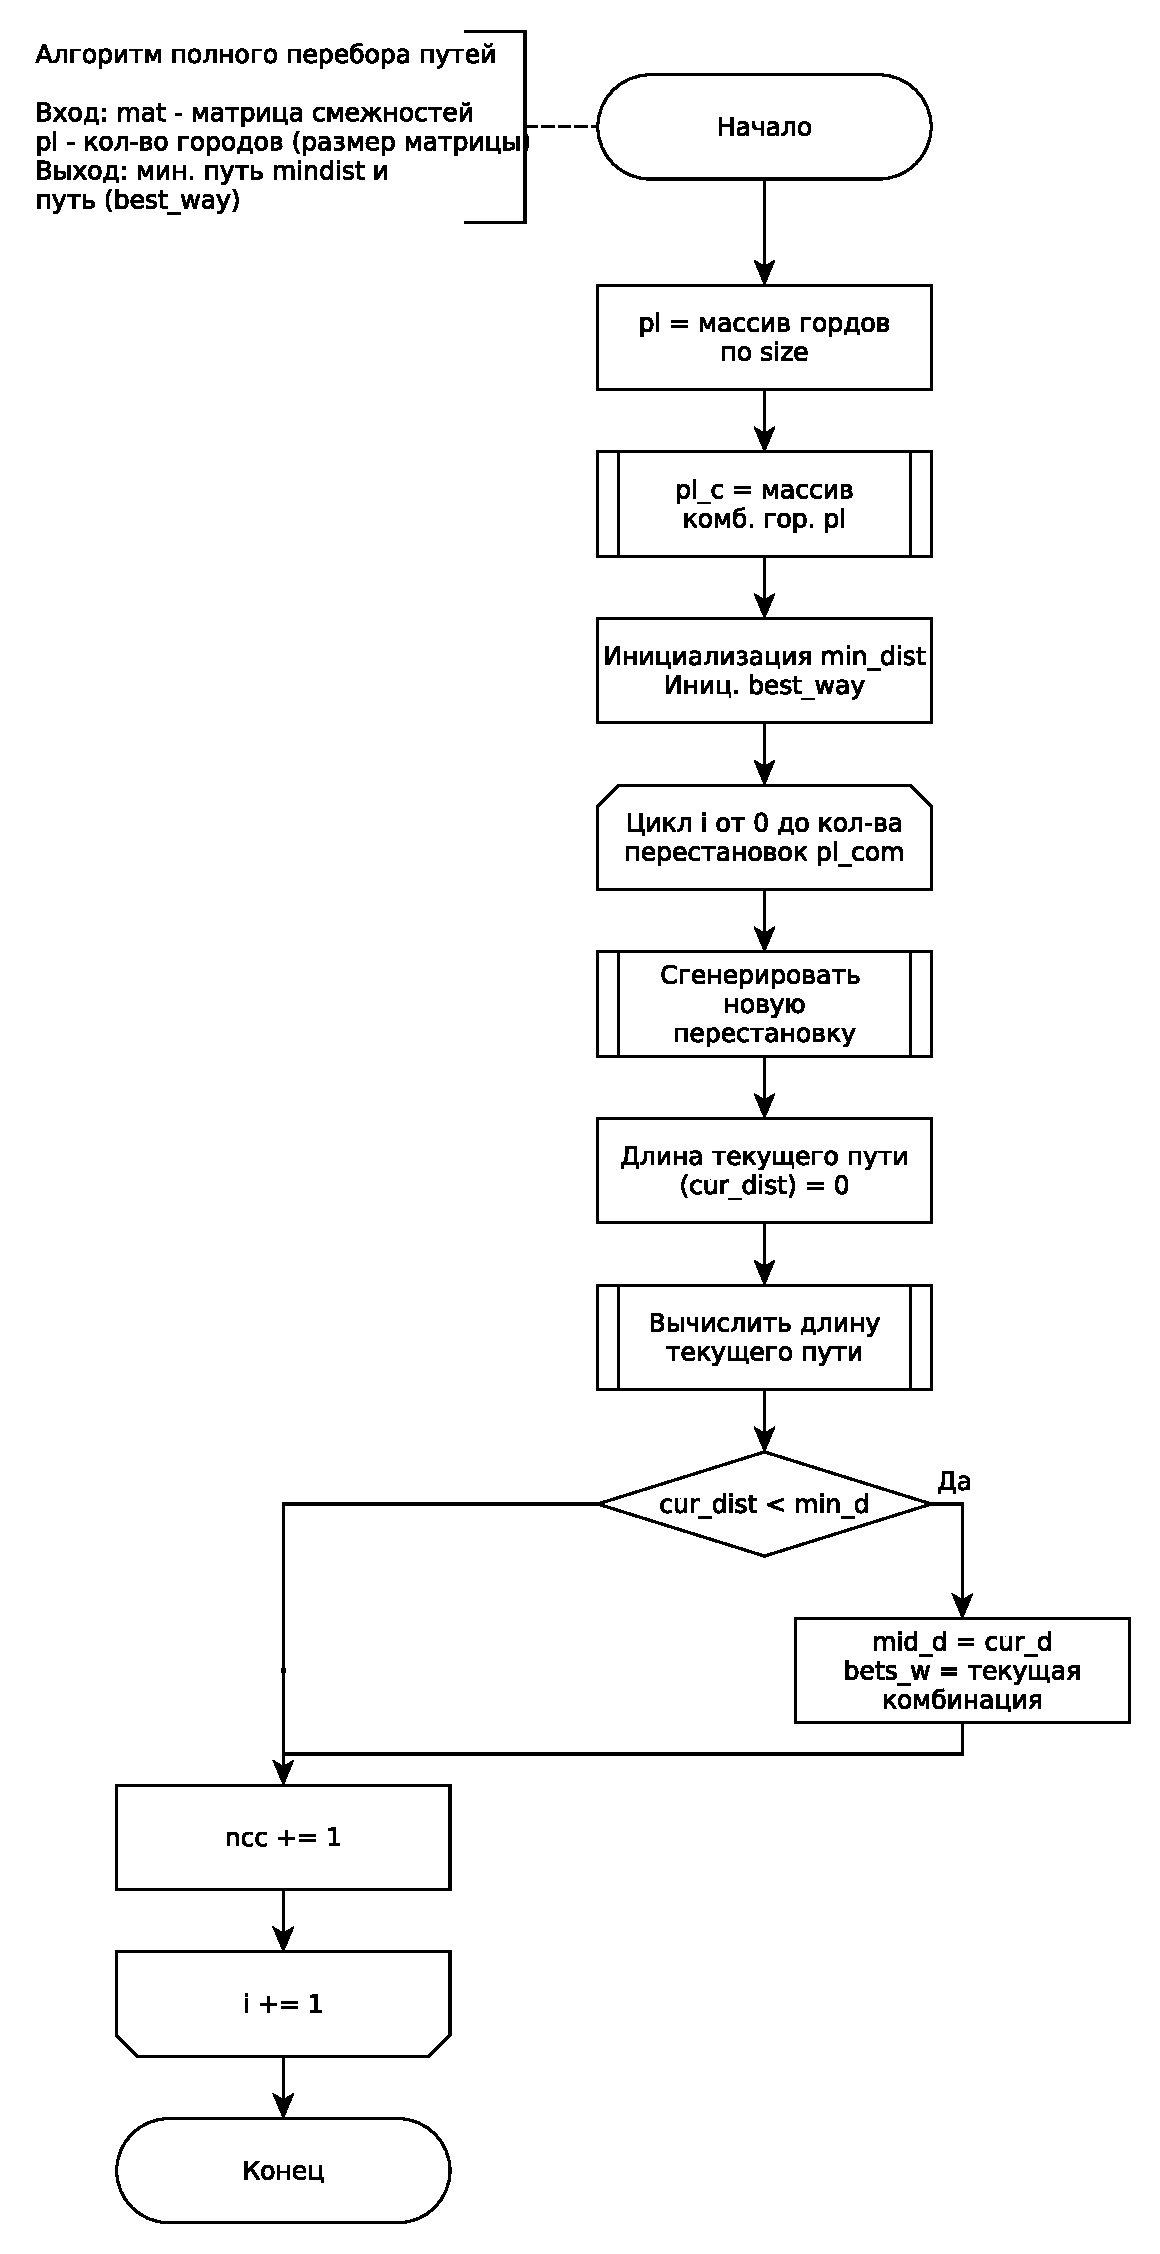
\includegraphics[width=0.7\linewidth]{assets/graphs/perebor.pdf}
	\caption{Схема алгоритма полного перебора путей}
	\label{fig:full_comb}
\end{figure}


\begin{figure}[ht!]
	\centering
	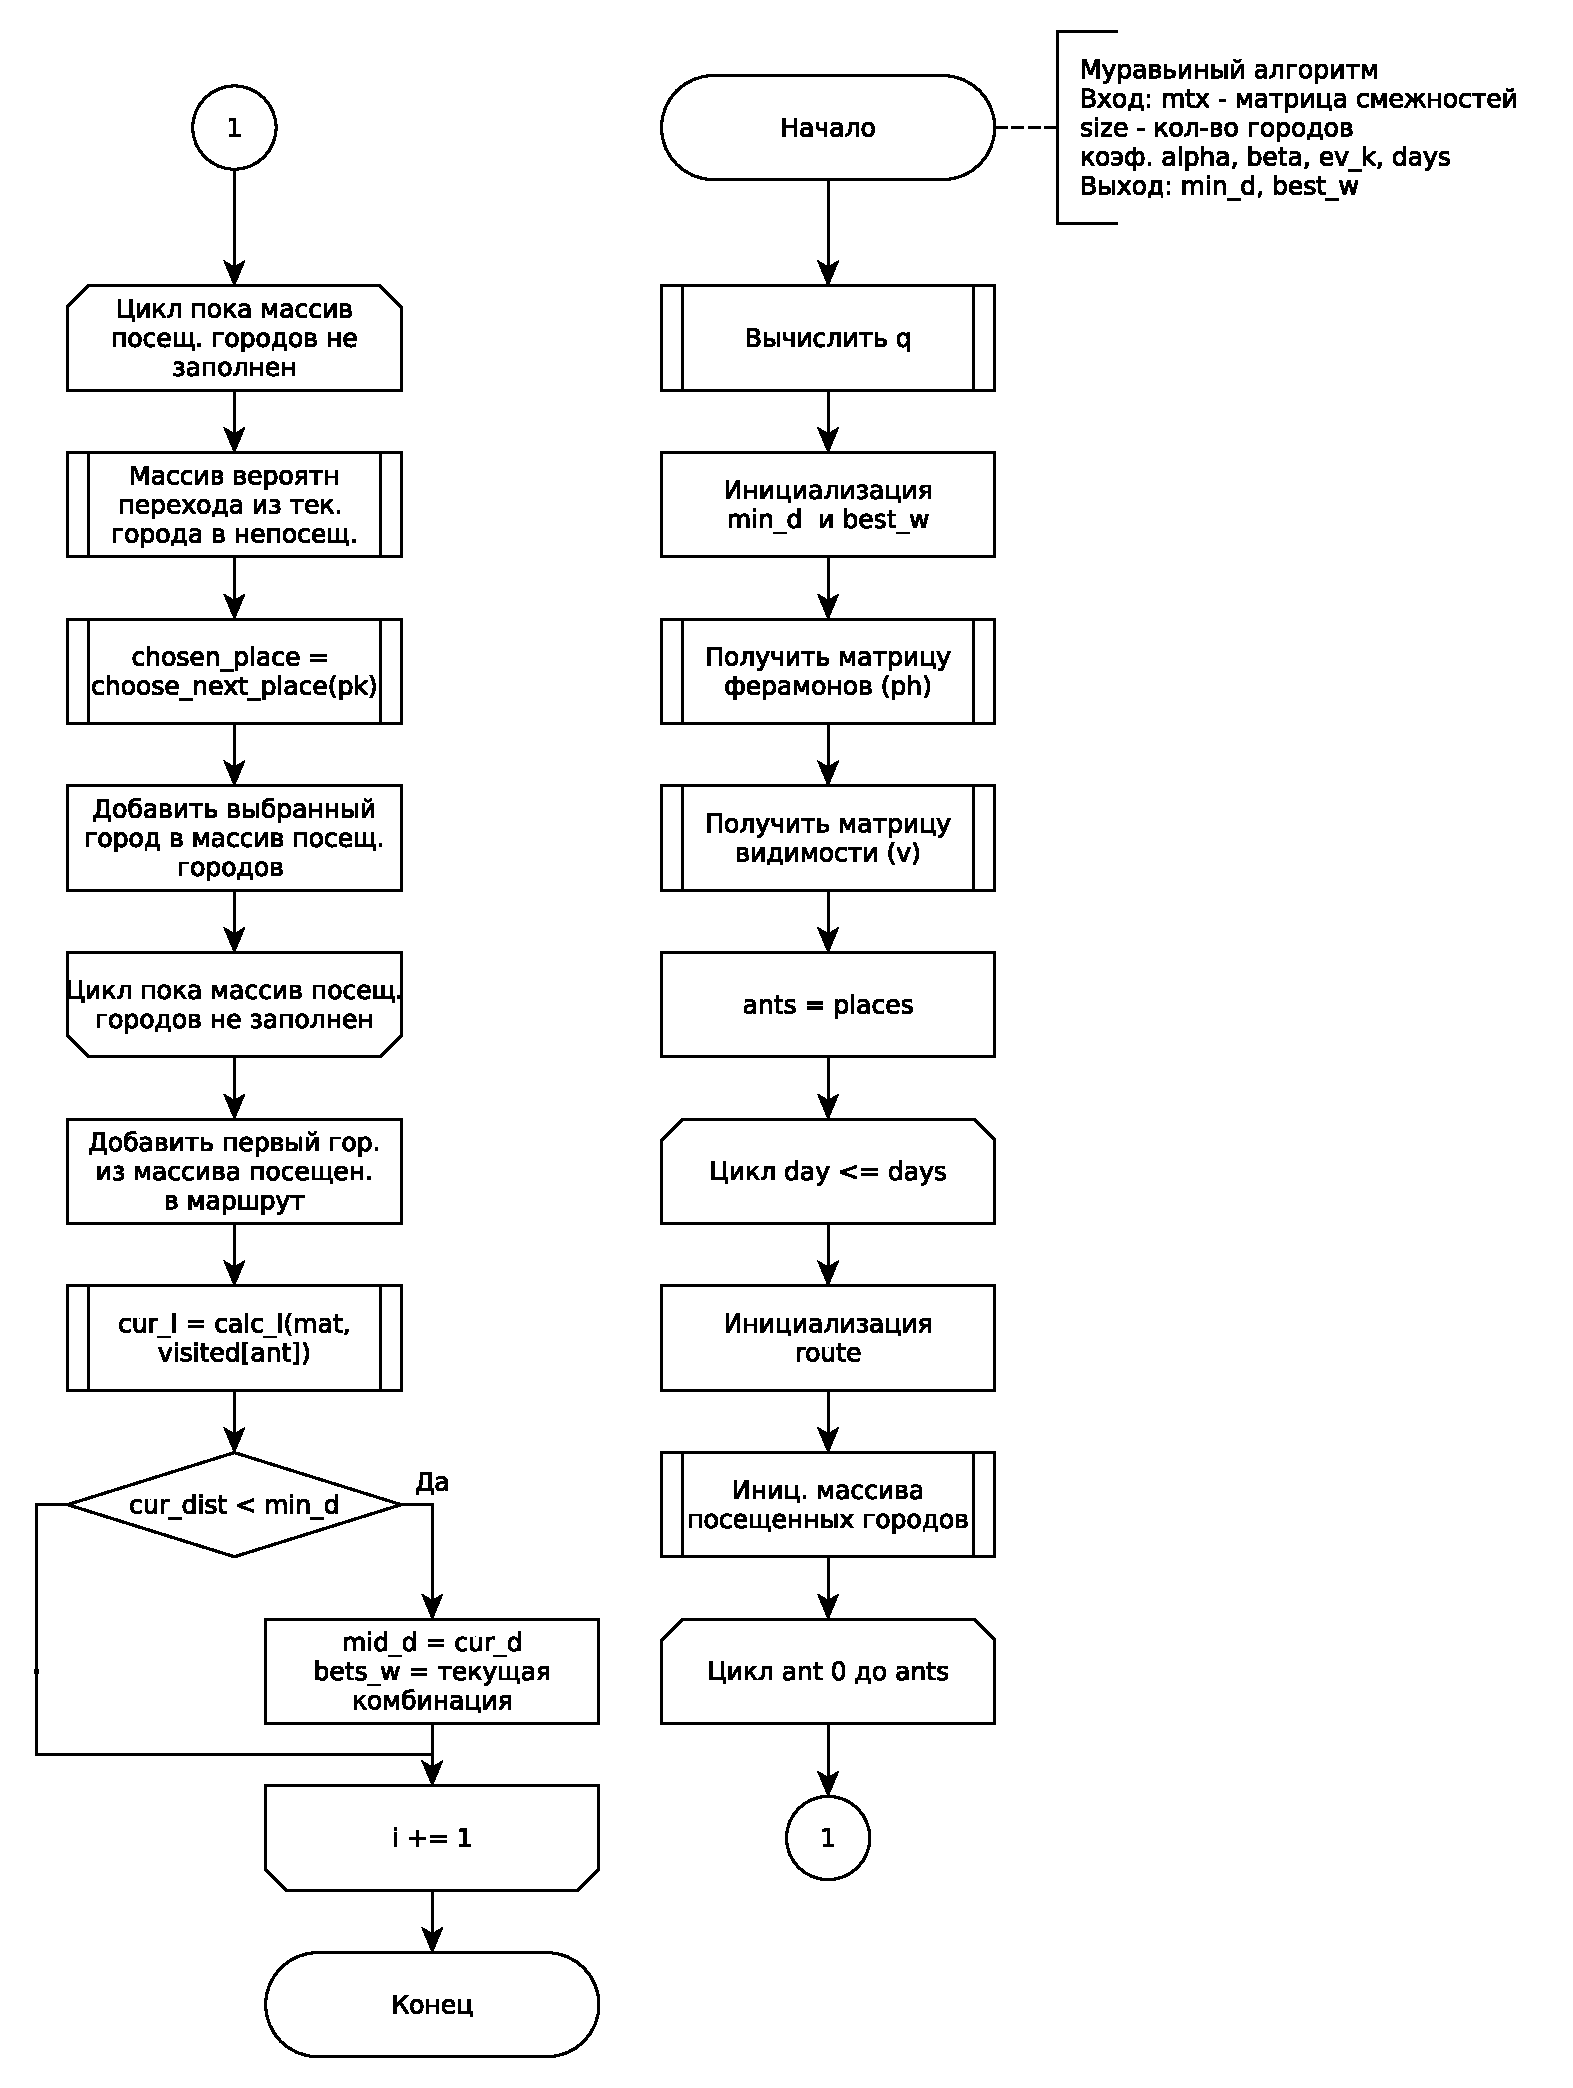
\includegraphics[width=1\linewidth]{assets/graphs/angs.pdf}
	\caption{Схема муравьиного алгоритма}
	\label{fig:angs}
\end{figure}


\begin{figure}[ht!]
	\centering
	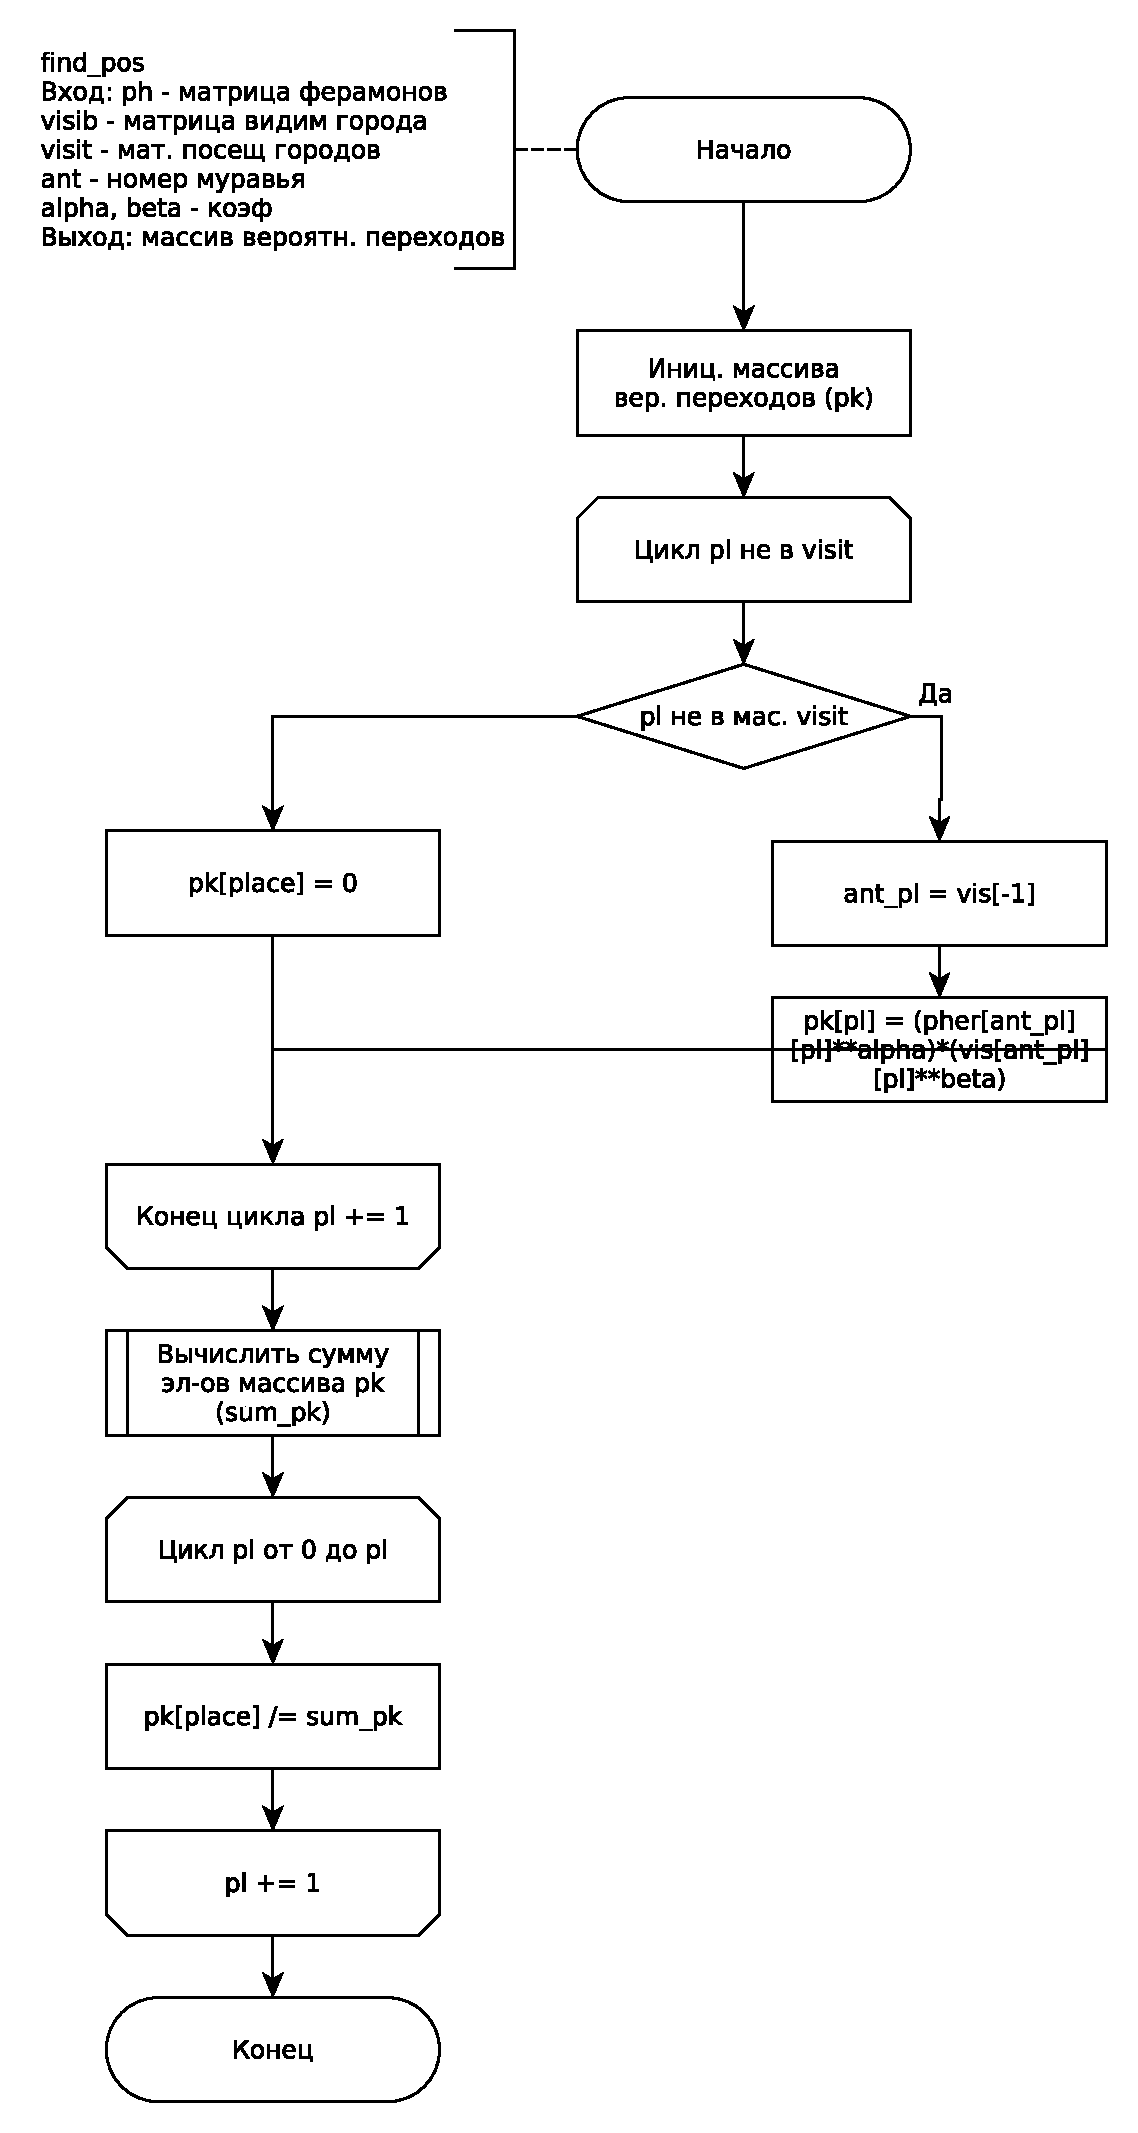
\includegraphics[width=0.8\linewidth]{assets/graphs/find_pos.pdf}
	\caption{Схема нахождения массива вероятностей переходов}
	\label{fig:find_pos}
\end{figure}

\begin{figure}[ht!]
	\centering
	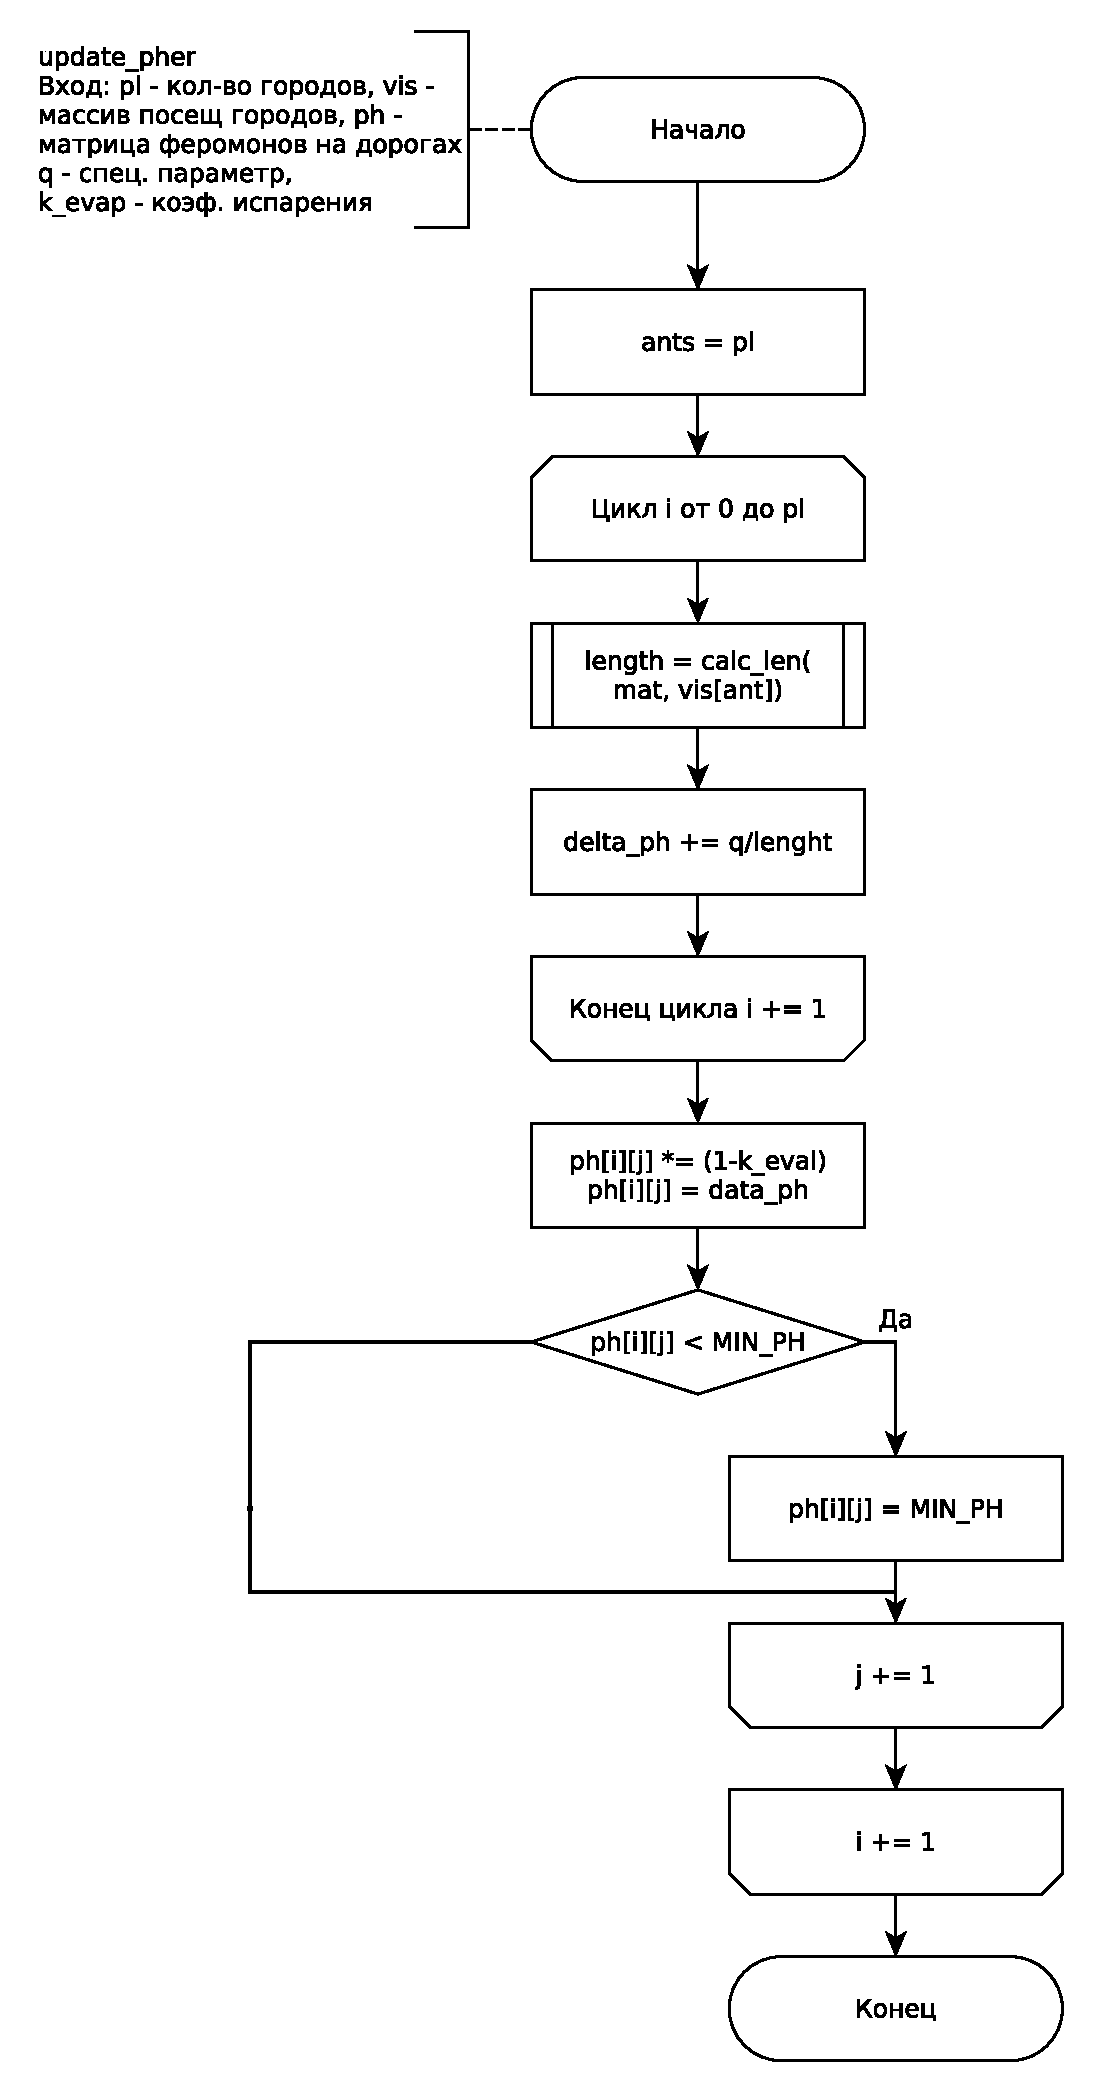
\includegraphics[width=0.750\linewidth]{assets/graphs/update_ph.pdf}
	\caption{Схема обновления матрицы феромонов}
	\label{fig:update_phero}
\end{figure}



\section*{Вывод}

Были разработаны схемы алгоритмов, необходимых для решения задачи.